\section{Results}
\label{sec:results}

The estimator recovers the truth when it is told the truth. Handing each
catalog only the events its objects actually host returns
$\Hz = \CtrlGalMedian$~\kmsmpc\ from the galaxies (\EvNhostGal\ events) and
$\Hz = \CtrlAgnMedian$~\kmsmpc\ from the AGN (\EvNhostAgn\ events), both
consistent with the input value: it lies inside the galaxy control's
68\% interval and the AGN control's 90\%. Section~\ref{sec:validation}
repeats this recovery across five independent realisations. The measurements that
follow use all \EvNobs\ events.

\subsection{The Hubble constant from one catalog at a time}
\label{sec:results:single}

\begin{figure}[t]
\centering
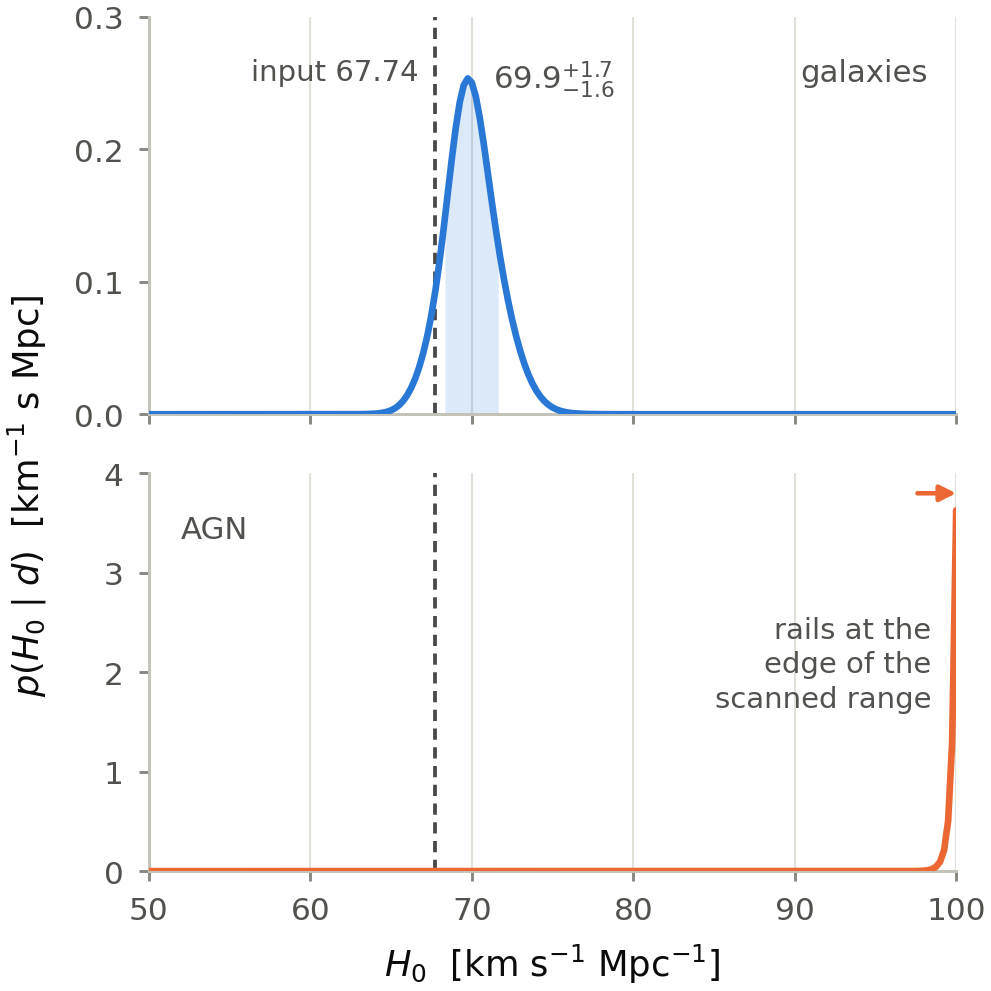
\includegraphics[width=\columnwidth]{figures/fig_single_tracer.pdf}
\caption{The same \EvNobs\ events analysed against one catalog at a time
(reference realisation, \Hz\ scanned over
$[\HzeroScanLo, \HzeroScanHi]$~\kmsmpc, the full range shown). Each panel
shows the normalised flat-prior posterior density $p(\Hz \mid d)$, in units
of km$^{-1}$\,s\,Mpc, for the galaxy catalog (top) and the AGN catalog
(bottom); the two panels share the \Hz\ axis, their density scales differ,
and no curve is rescaled. The dashed line is the input value, and the shaded
band is the galaxy analysis' 68\% interval, $\Hz = \HzeroGal$~\kmsmpc. The
AGN-only posterior has no interior maximum: it is still rising at the edge
of the scanned range, so no interval is quoted for it. Neither analysis knows
that the events were drawn from a mixture of the two catalogs.
\label{fig:single}}
\end{figure}

A single-catalog analysis asserts that every host is in that catalog, and in
this universe the assertion fails for both: the galaxy catalog is missing the
hosts of the \EvNhostAgn\ AGN-hosted events, and the AGN catalog those of the
\EvNhostGal\ galaxy-hosted ones. What differs is the price. From the galaxy
catalog alone we find $\Hz = \HzeroGal$~\kmsmpc\
(Figure~\ref{fig:single}): the input value lies within the 90\% interval but
outside the 68\%, whose full width is \HzeroGalWidth~\kmsmpc. The dense
catalog absorbs the events that do not belong to it at a modest price because
it offers many candidate hosts along every line of sight, tracing the same
structure the true hosts occupy.

The AGN catalog alone fails outright. Asked to explain \EvNobs\ events with a
catalog that hosts \EvNhostAgn\ of them, its posterior climbs into the upper
edge of the analysed range (median \HzeroAgnRailMedian\ against a boundary at
\HzeroScanHi~\kmsmpc), and we quote no interval from a posterior that peaks on
the boundary of its support. The asymmetry between the two catalogs has a
simple reading: sharp localisation cuts both ways. The sparse catalog pins its
own events to a handful of hosts, but by the same token it offers no diffuse
background of candidates that could plausibly absorb the \EvNhostGal\ events
that are not its to explain.

\subsection{The Hubble constant and the AGN-hosted fraction jointly}
\label{sec:results:joint}

\begin{figure*}[t]
\centering

\includegraphics[width=\textwidth]{figures/fig_joint.pdf}
\caption{Both parameters at once: the joint posterior on the two complete
catalogs with the mixture weight free. Blue: the reference realisation's 68\%
and 90\% highest-density credible regions, with the corresponding marginals
in the side panels. Gray: the 90\% regions and marginals of four further
realisations of the entire simulated universe. The cross marks the input
expansion rate and the reference realisation's realised hosted fraction
\FagnTruthReal\ (input value \FagnTruthPlanted; short gray ticks mark the other
realisations' realised fractions). Axes span the union of the realisations'
90\% regions, and the side panels share those axes and show the shapes of
the marginal posteriors, without a density scale. The recovered $\Hz = \HzeroJoint$~\kmsmpc\ interval is a
factor of \HzeroWidthRatio\ narrower than the galaxy-only interval of
Figure~\ref{fig:single}: the second catalog sharpens the expansion rate
rather than diluting it.
\label{fig:joint}}
\end{figure*}

Freeing the mixture removes the misassignment entirely. With both catalogs
entering through Equation~(\ref{eq:mixture}) and $(\Hz, \fagn)$ free, we find
$\Hz = \HzeroJoint$~\kmsmpc\ and $\fagn = \FagnJoint$
(Figure~\ref{fig:joint}): the realised hosted fraction lies inside the 68\%
interval, and the input expansion rate inside the 90\%, the same standing the
galaxy-only analysis reaches with a far wider interval. The two parameters
are only weakly correlated ($\rho = \JointRho$ here, $\JointRhoMean$ across
realisations), so little of the fraction is bought with expansion-rate
information. The reference against which \fagn\ should be
judged is the fraction actually realised, \FagnTruthReal, rather than the
input probability \FagnTruthPlanted: a draw of \EvNobs\ hosts scatters
binomially by \FagnBinomialSd, and the likelihood of a mixture weight peaks at
the fraction present in the data, not at the probability that generated it.

The joint fit is the sharpest of the analyses that use all \EvNobs\ events.
Its 68\% interval spans \HzeroJointWidth~\kmsmpc\ against \HzeroGalWidth\ for
the galaxy catalog alone (a factor of \HzeroWidthRatio), so adding a
catalog one hundred times sparser, and paying one new parameter for it,
sharpens the expansion rate rather than diluting it. We read the gain as an
assignment effect: once each event is allowed to belong to the catalog that
actually hosts it, the \EvNhostAgn\ AGN-hosted events are anchored by a
redshift prior concentrated in a few sharp structures instead of being spread
across the galaxy catalog's smooth one. The comparison mixes two effects,
the repair of the misassignment and the second catalog's own information.
Appendix~\ref{app:pure} measures the second directly: on events it actually
hosts, and at the same event count, the AGN catalog alone is a factor of
\PureWidthRatio\ sharper than the galaxy catalog.

A universe with no AGN channel is excluded. Profiled over \Hz, the likelihood
at $\fagn = 0$ falls \FagnZeroDlnL\ $e$-folds below its peak.

\subsection{Incomplete catalogs}
\label{sec:results:incomplete}

\begin{figure*}[t]
\centering
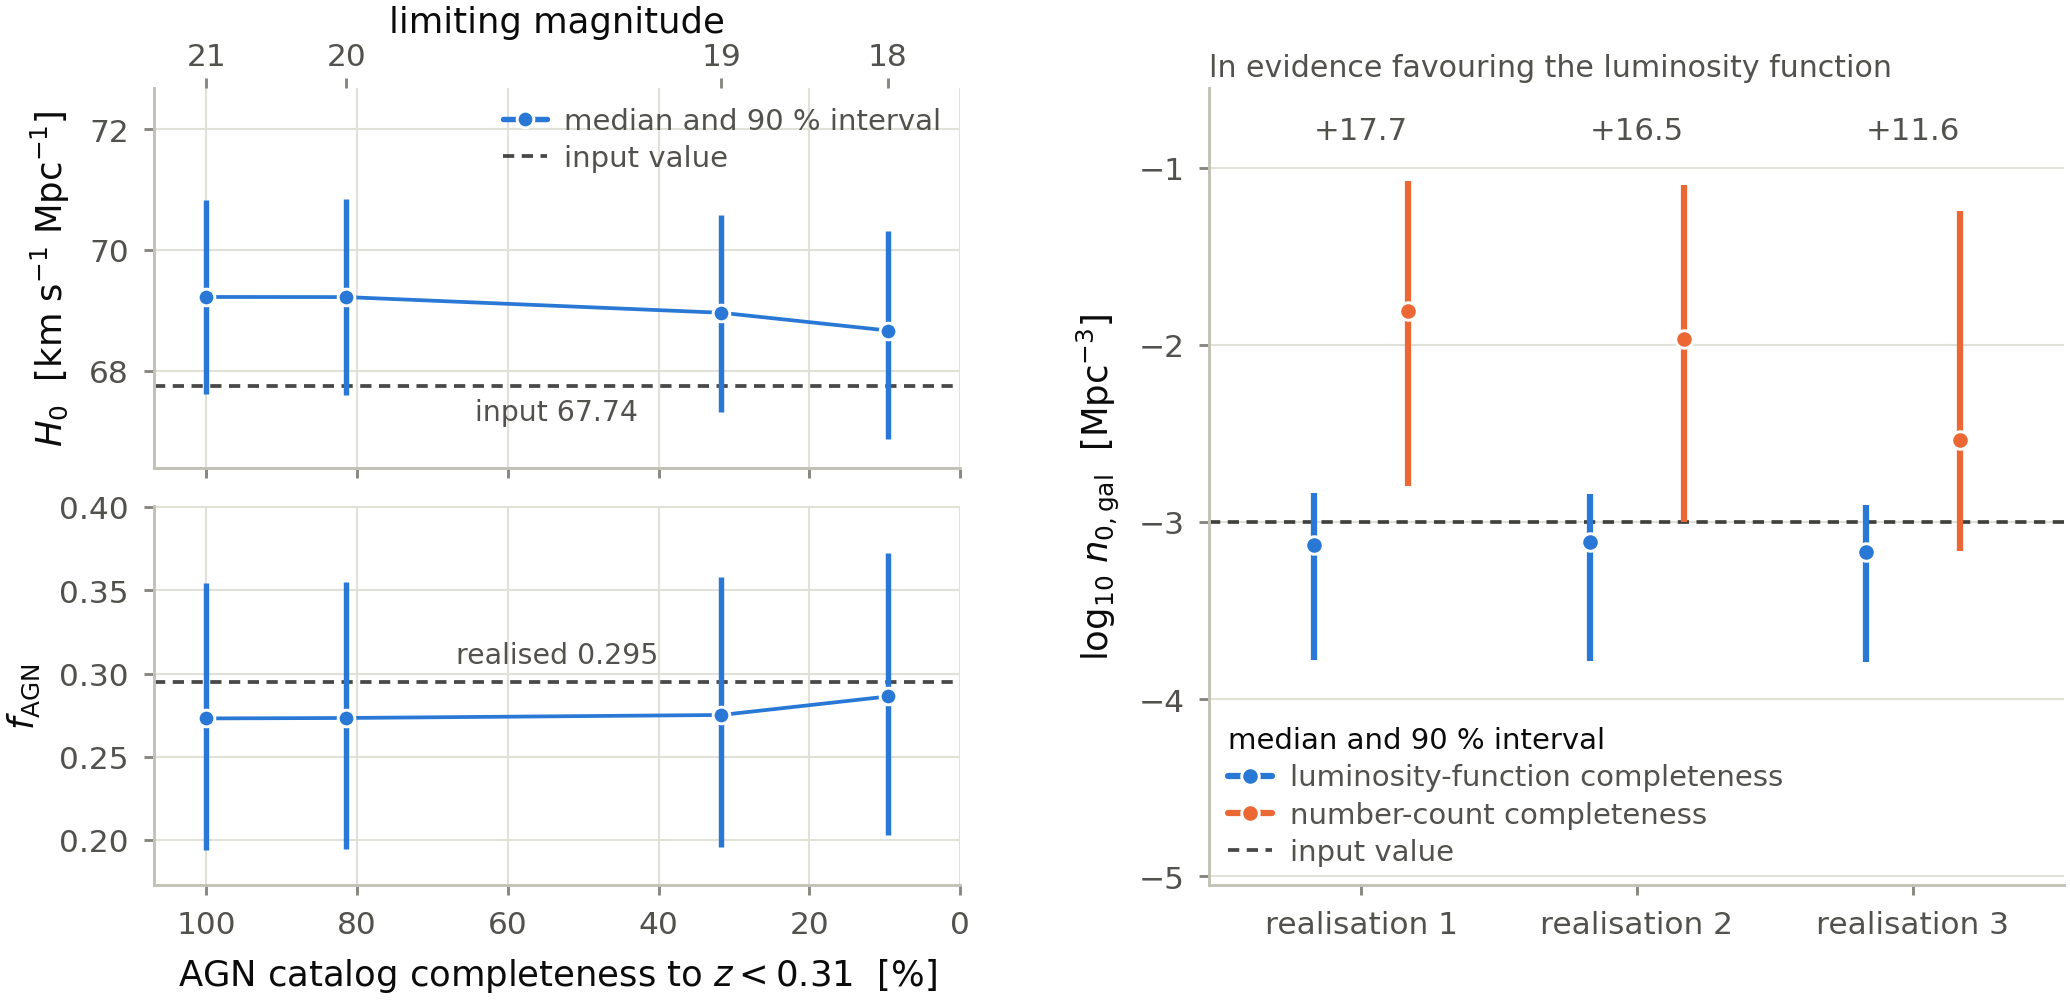
\includegraphics[width=\textwidth]{figures/fig_incomplete.pdf}
\caption{The joint measurement on flux-limited catalogs. Left: \Hz\ (upper)
and \fagn\ (lower) against the AGN catalog's completeness within the volume
the events occupy, with the corresponding magnitude limit on the upper
axis, the completeness of each catalog computed from its magnitude limit
and its luminosity function, and both number densities held at their input
values, on the reference realisation of the simulated universe. Points and
bars are medians with 90\% intervals; dashed lines mark the input expansion
rate and the realised hosted fraction. Right: the galaxy number density
recovered with both densities free at the shallowest limit, on three
independent realisations, under luminosity-function completeness and under
number-count completeness; bars are 90\% intervals, the dashed line is the
input value, and each annotation is that realisation's ln evidence
favouring the luminosity function. The number-count medians overstate the
density by \PixelAnchorBiasMinDex\ to \PixelAnchorBiasMaxDex~dex; the
luminosity-function intervals contain the input value in all three
realisations, the number-count intervals in one.
\label{fig:incomplete}}
\end{figure*}

A flux-limited survey removes hosts, and the mixture must complete both
catalogs to keep its weight meaningful. Repeating the joint fit on the
flux-limited catalogs of \S\ref{sec:data:survey}, with each catalog's
completeness computed from its magnitude limit and its luminosity function
(\S\ref{sec:methods:completion}) and both number densities held at their
input values, preserves the measurement at every depth on the reference
realisation (Figure~\ref{fig:incomplete}): the input \Hz\ lies inside the
90\% interval at the three deeper limits and the 68\% at the shallowest,
and \fagn\ holds the realised fraction inside the 68\% at all four. At the
shallowest limit, where \CompMEighteen\ per cent of hosts remain
catalogued, we find $\Hz = \HzeroIncomplete$~\kmsmpc\ and
$\fagn = \FagnIncomplete$, the \fagn\ interval essentially unchanged from
the complete catalogs (a factor of \FagnWidthRatio).

Anchoring the densities is the strongest assumption the completion makes,
and it can be dropped. Freeing both $n_{0,k}$ under flat priors at the
shallowest limit returns the galaxy density to within
\GalDensityFreeOffsetDex~dex of the input value, inside the 68\% interval
($\log_{10} n_0 = \GalDensityFree$); the widening falls almost entirely on
the fraction, whose interval grows by a factor of \FagnFreeWidthRatio\
($\fagn = \FagnFree$). In all three realisations the free-density \fagn\
median lies \FagnFreeOffsetMin\ to \FagnFreeOffsetMax\ above the reference
fraction, each inside its own 68\% interval; three realisations do not
resolve whether that offset is systematic. The dependence on the assumed
density is continuous rather than a cliff; at fixed depth, a one-dex error
in the assumed AGN density moves \fagn\ by \FagnDensitySlope. The fraction
is only as well determined as the AGN number density.

The completeness itself can be estimated two ways, from the survey's
selection or from the observed counts (\S\ref{sec:methods:completion}), and
the data distinguish them. Repeated on \NSeedsIncomplete\ independent
realisations at the shallowest limit with both densities free,
number-count completeness places the galaxy density \PixelAnchorBiasMinDex\
to \PixelAnchorBiasMaxDex~dex above the input, luminosity-function
completeness holds it within \GalAnchorOffsetMaxDex~dex with the input
inside the 68\% interval in every realisation, and the data prefer
luminosity-function completeness by \SeedLnBFmin\ to \SeedLnBFmax\
$e$-folds of evidence (Figure~\ref{fig:incomplete}, right).

\Hz\ is the robust parameter of the pair, within a stated limit. While the
catalogs remain at least \CompMTwenty\ per cent complete, a factor-of-two
error in the assumed AGN density moves \Hz\ by
\HzDensityShiftFactorTwoDeep~\kmsmpc; at \CompMEighteen\ per cent
completeness the same error displaces it by
\HzDensityShiftFactorTwo~\kmsmpc\ (\HzDensitySlopeShallow~\kmsmpc\ per
dex), half the complete-catalog interval of \HzeroJointWidth~\kmsmpc. A survey working at such depths must know the AGN
density it assumes, for the expansion rate and not only for the fraction.
